\chapter{Equazioni di Eulero-Lagrange e integrali primi del moto}

\section{Equazioni di Eulero-Lagrange}
\begin{lemma}{}
Consideriamo $n$ punti materiali $\underline{x}_1, \underline{x}_2, \ldots, \underline{x}_n$ soggetti a $3n - m$ vincoli olonomi. Supponiamo che il sistema sia rappresentato da $m$ coordinate libere $q_1(t), \ldots, q_m(t)$. Allora vale la relazione
\[
\frac{\partial \dot{\underline{x}}_i}{\partial \dot{q}_j}
=
\frac{\partial \underline{x}_i}{\partial q_j}
\qquad
\forall i = 1,\ldots,n,\quad \forall j = 1,\ldots,m .
\]
\end{lemma}
\begin{proof}
Ricordiamo che $\underline{x}_i(q_1,\ldots,q_m,t)$ dipende dalle coordinate libere ma non dalle loro derivate temporali, allora
\[
\frac{\partial \underline{x}_i}{\partial \dot{q}_j} = 0
\qquad \forall j = 1,\ldots,m .
\]

Quindi
\[
\frac{\partial \dot{\underline{x}}_i}{\partial \dot{q}_j}
=
\frac{\partial}{\partial \dot{q}_j}
\frac{d\underline{x}_i}{dt}
=
\frac{\partial}{\partial \dot{q}_j}
\sum_k
\frac{\partial \underline{x}_i}{\partial q_k}
\frac{dq_k}{dt}
=
\frac{\partial}{\partial \dot{q}_j}
\sum_k
\frac{\partial \underline{x}_i}{\partial q_k}
\dot{q}_k
\]
\[
=
\sum_k
\frac{\partial \underline{x}_i}{\partial q_k}
\frac{\partial \dot{q}_k}{\partial \dot{q}_j}
=
\sum_k
\frac{\partial \underline{x}_i}{\partial q_k}
\delta_{kj}
=
\frac{\partial \underline{x}_i}{\partial q_j}.
\]
\end{proof}

Scriviamo il principio dei lavori virtuali per il sistema descritto nel lemma aggiungendo il termine d'inerzia:
\[
\sum_{i=1}^{n} m_i \ddot{\underline{x}}_i \cdot \delta \underline{x}_i
=
\sum_{i=1}^{n} \underline{f}_i \cdot \delta \underline{x}_i
\qquad
\forall \left(\delta \underline{x}_1,\ldots,\delta \underline{x}_n\right).
\]

Dove $\delta \underline{x}_i$ è uno spostamento virtuale ammesso dai vincoli perfetti e olonomi per il punto $\underline{x}_i$. Come abbiamo già fatto in precedenza possiamo scrivere
\[
\sum_{i=1}^{n} \underline{f}_i \cdot \delta \underline{x}_i
=
\sum_{i=1}^{n} \underline{f}_i^{\mathrm{ATT}} \cdot \delta \underline{x}_i
=
\sum_{i=1}^{n} \underline{f}_i^{\mathrm{ATT}} \cdot
\sum_{j=1}^{m}
\frac{\partial \underline{x}_i}{\partial q_j}\delta q_j
=
\sum_{j=1}^{m}
\left(
\sum_{i=1}^{n}
\underline{f}_i^{\mathrm{ATT}} \cdot
\frac{\partial \underline{x}_i}{\partial q_j}
\right)\delta q_j
=
\sum_{j=1}^{m} Q_j \delta q_j.
\]

Inoltre
\[
\sum_{i=1}^{n} m_i \ddot{\underline{x}}_i \cdot \delta \underline{x}_i
=
\sum_{i=1}^{n} m_i \ddot{\underline{x}}_i \cdot
\sum_{j=1}^{m}
\frac{\partial \underline{x}_i}{\partial q_j}\delta q_j
=
\sum_{j=1}^{m}
\left(
\sum_{i=1}^{n}
m_i \ddot{\underline{x}}_i \cdot
\frac{\partial \underline{x}_i}{\partial q_j}
\right)\delta q_j.
\]

Ricordiamo che
\[
\left(\frac{d}{dt}f\right)\cdot g
=
\frac{d}{dt}(f\cdot g)
-
f\cdot \frac{d}{dt}(g).
\]
Allora
\[
\sum_{j=1}^{m}
\left(
\sum_{i=1}^{n}
m_i \ddot{\underline{x}}_i \cdot
\frac{\partial \underline{x}_i}{\partial q_j}
\right)\delta q_j
=
\sum_{j=1}^{m}
\left(
\sum_{i=1}^{n}
\left[
\frac{d}{dt}
\left(
m_i \dot{\underline{x}}_i \cdot
\frac{\partial \underline{x}_i}{\partial q_j}
\right)
-
m_i \dot{\underline{x}}_i \cdot
\frac{d}{dt}
\left(
\frac{\partial \underline{x}_i}{\partial q_j}
\right)
\right]
\right)\delta q_j.
\]

Ora applichiamo il lemma al primo
$
{\partial \underline{x}_i}/{\partial q_j}.
$

\[
\sum_{j=1}^{m}\sum_{i=1}^{n}
\left[
\frac{d}{dt}
\left(
m_i \dot{\underline{x}}_i \cdot
\frac{\partial \underline{ \dot x}_i}{\partial \dot q_j}
\right)
-
m_i \dot{\underline{x}}_i \cdot
\frac{\partial \dot{\underline{x}}_i}{\partial q_j}
\right]\delta q_j
=
\]
\[
=
\sum_{j=1}^{m}\sum_{i=1}^{n}
\left[
\frac{d}{dt}
\left(
m_i \underline{v}_i \cdot
\frac{\partial \underline{v}_i}{\partial \dot{q}_j}
\right)
-
m_i \underline{v}_i \cdot
\frac{\partial \underline{v}_i}{\partial q_j}
\right]\delta q_j
=
\]
\[
=
\sum_{j=1}^{m}
\left[
\frac{d}{dt}
\left(
\sum_{i=1}^{n}
m_i \underline{v}_i \cdot
\frac{\partial \underline{v}_i}{\partial \dot{q}_j}
\right)
-
\sum_{i=1}^{n}
m_i \underline{v}_i \cdot
\frac{\partial \underline{v}_i}{\partial q_j}
\right]\delta q_j
=
\]
\[
=
\sum_{j=1}^{m}
\left[
\frac{d}{dt}
\left(
\frac{\partial}{\partial \dot{q}_j}
\sum_{i=1}^{n}
m_i \frac{\underline{v}_i \cdot \underline{v}_i}{2}
\right)
-
\frac{\partial}{\partial q_j}
\left(
\sum_{i=1}^{n}
m_i \frac{\underline{v}_i \cdot \underline{v}_i}{2}
\right)
\right]\delta q_j
=
\]
\[
=
\sum_{j=1}^{m}
\left[
\frac{d}{dt}
\frac{\partial T}{\partial \dot{q}_j}
-
\frac{\partial T}{\partial q_j}
\right]\delta q_j.
\]

Mettendo assieme i due membri otteniamo
\[
\sum_{j=1}^{m}
\left[
\frac{d}{dt}
\frac{\partial T}{\partial \dot{q}_j}
-
\frac{\partial T}{\partial q_j}
\right]\delta q_j
=
\sum_{j=1}^{m} Q_j \delta q_j
\qquad
\forall (\delta q_1,\ldots,\delta q_m).
\]

\[
\Rightarrow \sum_{j=1}^{m}
\left[
\frac{d}{dt}
\frac{\partial T}{\partial \dot{q}_j}
-
\frac{\partial T}{\partial q_j}
-
Q_j
\right]\delta q_j
=
0
\qquad
\forall (\delta q_1,\ldots,\delta q_m).
\]

\[
\Rightarrow \begin{pmatrix}
\frac{d}{dt}\frac{\partial T}{\partial \dot{q}_1}
-
\frac{\partial T}{\partial q_1}
-
Q_1
\\
\vdots
\\
\frac{d}{dt}\frac{\partial T}{\partial \dot{q}_m}
-
\frac{\partial T}{\partial q_m}
-
Q_m
\end{pmatrix}
\cdot
\begin{pmatrix}
\delta q_1
\\
\vdots
\\
\delta q_m
\end{pmatrix}
=
0
\qquad
\forall (\delta q_1,\ldots,\delta q_m).
\]

\[
\Rightarrow \frac{d}{dt}
\frac{\partial T}{\partial \dot{q}_j}
-
\frac{\partial T}{\partial q_j}
-
Q_j
=
0
\qquad
\forall j = 1,\ldots,m.
\]

\[
\Rightarrow \frac{d}{dt}
\frac{\partial T}{\partial \dot{q}_j}
-
\frac{\partial T}{\partial q_j}
=
Q_j
\qquad
\forall j = 1,\ldots,m.
\]
Chiamiamo queste ultime equazioni \textbf{equazioni di Eulero-Lagrange} o più semplicemente \textbf{equazioni di Lagrange}. Le \textbf{equazioni di Lagrange} sono $m$ equazioni (per un sistema con $m$ gradi di libertà) del $II$ ordine nel tempo. Nelle equazioni non compaiono le reazioni vincolari.

Consideriamo ora un sistema sul quale agiscono solo forze conservative:
\[
Q_j
=
\sum_{i=1}^{n}
\underline{f}_i^{\mathrm{ATT}}
\cdot
\frac{\partial \underline{x}_i}{\partial q_j}
=
\sum_{i=1}^{n}
-\nabla V_i
\cdot
\frac{\partial \underline{x}_i}{\partial q_j}
=
\sum_{i=1}^{n}
-
\begin{pmatrix}
\frac{\partial V_i}{\partial x_i}
\\[2pt]
\frac{\partial V_i}{\partial y_i}
\\[2pt]
\frac{\partial V_i}{\partial z_i}
\end{pmatrix}
\cdot
\frac{\partial \underline{x}_i}{\partial q_j}
=
\]
\[
=
\sum_{i=1}^{n}
-
\frac{\partial V_i}{\partial q_j}
=
-
\frac{\partial V}{\partial q_j}.
\]

Allora
\[
\frac{d}{dt}
\frac{\partial T}{\partial \dot{q}_j}
-
\frac{\partial T}{\partial q_j}
=
-
\frac{\partial V}{\partial q_j}
\quad \Longrightarrow \quad
\frac{d}{dt}
\frac{\partial T}{\partial \dot{q}_j}
-
\frac{\partial}{\partial q_j}
(T - V)
=
0.
\]

Dal momento che
\[
\frac{\partial V}{\partial \dot{q}_j} = 0
\]
possiamo scrivere
\[
\frac{d}{dt}
\frac{\partial}{\partial \dot{q}_j}
(T - V)
-
\frac{\partial}{\partial q_j}
(T - V)
=
0.
\]

Chiamiamo ora funzione lagrangiana la funzione
\[
\mathcal{L}(\underline{q},\dot{\underline{q}})
=
T(\underline{q},\dot{\underline{q}})
-
V(\underline{q}).
\]

Otteniamo infine
\[
\frac{d}{dt}
\frac{\partial \mathcal{L}}{\partial \dot{q}_j}
-
\frac{\partial \mathcal{L}}{\partial q_j}
=
0. \quad \forall j = 1, \ldots , m
\]

ovvero le \textbf{equazioni di Lagrange per sistemi conservativi}.



\begin{example}{}
Vogliamo studiare la dinamica del sistema in figura. Farlo attraverso le equazioni cardinali è molto complesso. Dal momento che agiscono solo forze conservative, può essere vantaggioso usare le equazioni di Lagrange.
\begin{center}
    \begin{tikzpicture}[
    x=1cm,
    y=1cm,
    >=Latex,
    line cap=round,
    line join=round,
    every node/.style={font=\small}
]

% Parametri
\def\R{1.55}

% Coordinate
\coordinate (O) at (0,0);
\coordinate (A) at (0,3.45);
\coordinate (G) at (7.20,\R);
\coordinate (C) at (7.20,0);
\coordinate (Top) at ($(G)+(0,\R)$);
\coordinate (B) at ($(A)!0.42!(G)$);

% Assi
\draw[black, line width=1.4pt, ->] (0,0) -- (10.2,0) node[below right] {$x$};
\draw[black, line width=1.4pt, ->] (0,0) -- (0,4.2) node[above left] {$y$};

% Parete verticale
\draw[black, line width=2pt] (0,0) -- (0,4.05);

% Origine
\node[below left] at (O) {$O$};

% Riferimento centrato in O
\draw[orange!85!black, line width=1.4pt, ->] (O) -- ++(0.95,0);
\draw[orange!85!black, line width=1.4pt, ->] (O) -- ++(0,0.95);
\node[orange!85!black, below] at ($(O)+(0.48,0)$) {$\underline{\imath}$};
\node[orange!85!black, left] at ($(O)+(0,0.48)$) {$\underline{\jmath}$};

\draw[orange!85!black, line width=1.2pt] (-0.45,0.18) circle (0.18);
\fill[orange!85!black] (-0.45,0.18) circle (0.03);
\node[orange!85!black, left] at (-0.62,0.62) {$\underline{k}$};

% Sbarrette verticali attaccate all'asse y
\draw[black, line width=1.6pt] (0,3.14) -- (0,3.56);
\draw[black, line width=1.6pt] (0.12,3.14) -- (0.12,3.56);

% Punto A
\node[left] at (A) {$A$};

% Asta
\draw[black, line width=1.8pt] (A) -- (G);

% Punto B
\fill[red] (B) circle (2.8pt);
\node[above] at (B) {$B$};

% Etichetta asta
\node[above right] at ($(B)!0.52!(G)$) {$l,m$};

% Angolo theta
\draw[black, line width=1.1pt]
($(A)+(0,-0.78)$) arc[start angle=-90,end angle=-14.5,radius=0.78];
\node at ($(A)+(0.72,-0.87)$) {$\theta$};

% Freccia verde in A
\draw[green!55!black, line width=1.4pt, ->] ($(A)$) -- ++(1.80,0);
\node[green!55!black, above] at ($(A)+(1.25,0.20)$) {$\underline{\psi}$};

% Molla attaccata all'asse y
\draw[black, line width=1.4pt, smooth, samples=240, domain=0:7.02]
plot (\x,{1.55 + 0.10*sin(900*\x)});

% Ruota
\draw[black, line width=1.8pt] (G) circle (\R);

% Punto C
\node[below] at (C) {$C$};

% Centro G
\filldraw[white, draw=black, line width=1.2pt] (G) circle (0.09);
\node[above left] at ($(G)+(-0.10,0.08)$) {$G$};

% Etichetta M,R
\node[above right] at ($(Top)+(0.95,-0.05)$) {$M,R$};

% Raggi tratteggiati
\draw[black, dashed, line width=1.1pt] (Top) -- (G);
\draw[black, dashed, line width=1.1pt] (G) -- ++(0.95,1.00);

% Angolo phi
\draw[black, line width=1.0pt, ->]
($(G)+(0,0.58)$) arc[start angle=90,end angle=46,radius=0.58];
\node at ($(G)+(0.47,0.92)$) {$\varphi$};

% Forza mg in B
\draw[red!85!black, line width=1.5pt, ->] (B) -- ++(0,-1.15);
\node[red!85!black, left] at ($(B)+(0.10,-0.70)$) {$m\underline{g}$};

% Forza Mg in G
\draw[red!85!black, line width=1.5pt, ->] (G) -- ++(0,-1.05);
\node[red!85!black, right] at ($(G)+(0.52,-0.62)$) {$M\underline{g}$};

% Forza elastica
\draw[red!85!black, line width=1.5pt, ->] (G) -- ++(-1.25,0);
\node[red!85!black, below] at ($(G)+(-0.82,-0.12)$) {$-k\,\underline{x}_G$};

% Assi verdi vicino a C
\draw[green!55!black, line width=1.4pt, ->] ($(C)+(0.18,0)$) -- ++(1.90,0);
\draw[green!55!black, line width=1.4pt, ->] ($(C)+(0.18,0)$) -- ++(0,0.95);
\node[green!55!black, right] at ($(C)+(2.10,0)$) {$\underline{\xi}_x$};
\node[green!55!black, right] at ($(C)+(0.22,0.58)$) {$\underline{\xi}_y$};

\end{tikzpicture}
  \end{center}
Come al solito usiamo come coordinata libera $\theta$ e supponiamo $\theta(0)=0$ e $x_G(0)=0$. Allora
\[
x_G = \ell \sin\theta,
\qquad
\dot{x}_G = \ell \cos\theta \dot{\theta},
\]
\[
y_G = R,
\qquad
\dot{y}_G = 0,
\]
\[
x_A = \frac{\ell}{2}\sin\theta,
\qquad
\dot{x}_A = \frac{\ell}{2}\cos\theta \dot{\theta},
\]
\[
y_A = R + \frac{\ell}{2}\cos\theta,
\qquad
\dot{y}_A = -\frac{\ell}{2}\sin\theta \dot{\theta}.
\]

L'energia cinetica totale è
\[
T = T^{\mathrm{asta}} + T^{\mathrm{disco}}.
\]

Per l'asta:
\[
T^{\mathrm{asta}}
=
\frac{m}{2}\frac{\ell^2}{4}\dot{\theta}^2
+
I_A^{\mathrm{asta}}\frac{\dot{\theta}^2}{2}
=
\frac{m}{2}\frac{\ell^2}{4}\dot{\theta}^2
+
\frac{m\ell^2}{12}\frac{\dot{\theta}^2}{2}
=
\frac{m\ell^2}{3}\frac{\dot{\theta}^2}{2}.
\]

Dalla relazione cinematica:
\[
\ell \sin\theta = R\psi
\quad \Longrightarrow \quad
\psi = \frac{\ell}{R}\sin\theta
\quad \Longrightarrow \quad
\dot{\psi} = \frac{\ell}{R}\cos\theta \dot{\theta}.
\]

Per il disco:
\[
T^{\mathrm{disco}}
=
\left(I_G + MR^2\right)\frac{\dot{\psi}^2}{2}
=
\frac{3}{2}MR^2\frac{\dot{\psi}^2}{2}
=
\frac{3}{2}MR^2\frac{1}{2}
\frac{\ell^2}{R^2}\cos^2\theta \dot{\theta}^2
=
\frac{3}{4}M\ell^2\cos^2\theta \dot{\theta}^2.
\]

L'energia potenziale è
\[
V
=
mg y_A + Mg y_G + \frac{K}{2}x_G^2
=
mg\left(R+\frac{\ell}{2}\cos\theta\right)
+
MgR
+
\frac{K}{2}\left(\ell \sin\theta\right)^2.
\]

Quindi la lagrangiana è
\[
\mathcal{L}
=
T - V
=
\frac{m\ell^2}{3}\frac{\dot{\theta}^2}{2}
+
\frac{3}{4}M\ell^2\cos^2\theta \dot{\theta}^2
-
mg\left(R+\frac{\ell}{2}\cos\theta\right)
-
MgR
-
\frac{K}{2}\left(\ell \sin\theta\right)^2.
\]

Calcoliamo:
\[
\frac{\partial \mathcal{L}}{\partial \dot{\theta}}
=
\frac{m\ell^2}{3}\dot{\theta}
+
\frac{3}{2}M\ell^2\cos^2\theta \dot{\theta},
\]
\[
\frac{\partial \mathcal{L}}{\partial \theta}
=
-\frac{3}{2}M\ell^2\dot{\theta}^2\cos\theta\sin\theta
+
mg\frac{\ell}{2}\sin\theta
-
K\ell^2\sin\theta\cos\theta.
\]

Inoltre
\[
\frac{d}{dt}
\frac{\partial \mathcal{L}}{\partial \dot{\theta}}
=
\frac{m\ell^2}{3}\ddot{\theta}
+
\frac{3}{2}M\ell^2\cos^2\theta \ddot{\theta}
-
3M\ell^2\cos\theta\sin\theta \dot{\theta}^2.
\]

Dall'equazione di Lagrange
\[
\frac{d}{dt}
\frac{\partial \mathcal{L}}{\partial \dot{\theta}}
-
\frac{\partial \mathcal{L}}{\partial \theta}
=
0
\]
otteniamo
\[
\frac{m\ell^2}{3}\ddot{\theta}
+
\frac{3}{2}M\ell^2\cos^2\theta \ddot{\theta}
-
3M\ell^2\cos\theta\sin\theta \dot{\theta}^2
+
\frac{3}{2}M\ell^2\dot{\theta}^2\cos\theta\sin\theta
-
mg\frac{\ell}{2}\sin\theta
+
K\ell^2\sin\theta\cos\theta
=
0.
\]
Questa è un'equazione del II ordine e va risolta numericamente.
\end{example}



\begin{example}{}
    Facciamo lo stesso con questo sistema.
    \begin{center}
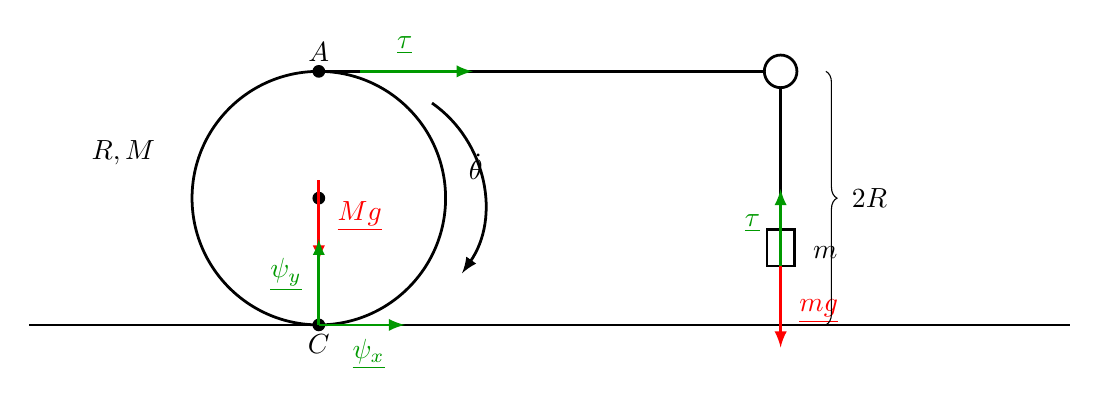
\begin{tikzpicture}[scale=1.15,>=latex]

% parametri
\def\R{1.4}

% piano
\draw[line width=1pt] (-3.2,0) -- (8.3,0);

% disco
\draw[line width=1pt] (0,\R) circle (\R);
\fill (0,\R) circle (2pt);

% punti A e C
\fill (0,2*\R) circle (2pt);
\fill (0,0) circle (2pt);
\node[above] at (0,2*\R) {\(A\)};
\node[below] at (0,0) {\(C\)};

% etichetta R,M
\node[left] at (-1.7,1.9) {\(R,M\)};

% peso disco
\draw[red,->,line width=1pt] (0,\R+0.2) -- (0,\R-0.7);
\node[red,right] at (0.1,\R-0.2) {\(\underline{Mg}\)};

% reazioni al contatto
\draw[green!60!black,->,line width=1pt] (0,0) -- (0.95,0);
\node[green!60!black,below] at (0.55,-0.05) {\(\underline{\psi_x}\)};

\draw[green!60!black,->,line width=1pt] (0,0) -- (0,0.95);
\node[green!60!black,left] at (-0.08,0.55) {\(\underline{\psi_y}\)};

% filo orizzontale e piolo
\draw[line width=1pt] (0,2*\R) -- (4.9,2*\R);
\draw[line width=1pt] (5.1,2*\R) circle (0.18);
\draw[line width=1pt] (5.1,2*\R-0.18) -- (5.1,1.05);

% massa appesa
\draw[line width=1pt] (4.95,1.05) rectangle (5.25,0.65);
\node[right] at (5.35,0.8) {\(m\)};

% tensioni
\draw[green!60!black,->,line width=1pt] (0.45,2*\R) -- (1.7,2*\R);
\node[green!60!black,above] at (0.95,2*\R+0.08) {\(\underline{\tau}\)};

\draw[green!60!black,->,line width=1pt] (5.1,0.65) -- (5.1,1.5);
\node[green!60!black,left] at (4.98,1.12) {\(\underline{\tau}\)};

% peso massa
\draw[red,->,line width=1pt] (5.1,0.65) -- (5.1,-0.25);
\node[red,right] at (5.2,0.15) {\(\underline{mg}\)};

% freccia di rotazione esterna al disco
\draw[->,line width=1pt] (1.25,2.45) arc[start angle=55,end angle=-35,radius=1.35];
\node[right] at (1.55,1.75) {\(\dot{\theta}\)};

% quota 2R
\draw[decorate,decoration={brace,amplitude=4pt}] (5.6,2*\R) -- (5.6,0);
\node[right] at (5.78,\R) {\(2R\)};

\end{tikzpicture}
\end{center}
Le energie cinetica e potenziale del sistema sono
\[
T
=
\frac{3}{2}MR^2\frac{\dot{\theta}^2}{2}
+
\frac{m}{2}\dot{y}_m^2,
\qquad
V
=
mg y_m + MgR.
\]

Ora, visto che
\[
v_A = 2R\dot{\theta}
\quad \Longrightarrow \quad
\dot{y}_m = -2R\dot{\theta},
\qquad
y_m = -2R\theta + h_0.
\]

Allora
\[
T
=
\frac{3}{2}MR^2\frac{\dot{\theta}^2}{2}
+
\frac{m}{2}4R^2\dot{\theta}^2
=
\dot{\theta}^2R^2
\left(
2m+\frac{3}{4}M
\right),
\]
\[
V
=
-2mgR\theta + MgR + mgh_0.
\]

Quindi
\[
\mathcal{L}
=
T - V
=
\dot{\theta}^2R^2
\left(
2m+\frac{3}{4}M
\right)
+
2mgR\theta
-
MgR
-
mgh_0.
\]

Dall'equazione di Lagrange
\[
\frac{d}{dt}
\frac{\partial \mathcal{L}}{\partial \dot{\theta}}
-
\frac{\partial \mathcal{L}}{\partial \theta}
=
0
\]
otteniamo
\[
\left(
\frac{3}{2}MR^2 + 4mR^2
\right)\ddot{\theta}
-
2mgR
=
0.
\]

Quindi
\[
\ddot{\theta}
=
\frac{2mgR}{\frac{3}{2}MR^2+4mR^2}
=
\frac{2mg}{\frac{3}{2}MR+4mR}
=
\frac{4mg}{3MR+8mR}.
\]

Infine
\[
\theta(t)
=
\frac{4mg}{3MR+8mR}
\frac{t^2}{2}.
\]

Che è lo stesso risultato che avevamo ottenuto con le equazioni cardinali.
\end{example}


\section{Integrali primi del moto}

\begin{definition}{}
Un \textbf{integrale primo del moto} è una combinazione delle coordinate libere e delle loro derivate, che resta costante nel tempo.
\end{definition}

\begin{example}{}
\begin{enumerate}[label=\roman*)]
\item Prima equazione cardinale con forze lungo $x$ nulle:
\[
\frac{d}{dt}\left(m\dot{x}_G\right)=0
\quad \Longrightarrow \quad
m\dot{x}_G(q_1,\ldots,q_m,\dot{q}_1,\ldots,\dot{q}_m)
=
\mathrm{cost.}
\]
In questo caso $m\dot{x}_G$ è un integrale primo del moto.

\item Seconda equazione cardinale con momenti nulli lungo $z$:
\[
\frac{d}{dt}\left(I_G\omega_z\right)=0
\quad \Longrightarrow \quad
I_G\omega_z(q_1,\ldots,q_m,\dot{q}_1,\ldots,\dot{q}_m)
=
\mathrm{cost.}
\]

\item Equazioni di Lagrange.

Supponiamo che
\[
\mathcal{L}(q_1,\ldots,q_m,\dot{q}_1,\ldots,\dot{q}_m)
\]
non dipenda da $q_j$ per un certo $j$. Allora
\[
\frac{d}{dt}
\frac{\partial \mathcal{L}}{\partial \dot{q}_j}
=
\frac{\partial \mathcal{L}}{\partial q_j}
=
0
\quad \Longrightarrow \quad
\frac{\partial \mathcal{L}}{\partial \dot{q}_j}
\]
è un integrale primo del moto.
\end{enumerate}
\end{example}

\begin{example}{}
Nel caso del pendolo che abbiamo studiato, la relazione
\[
E(\theta,\dot{\theta})=\mathrm{cost.}
\]
è un integrale primo del moto.

L'esistenza di un integrale primo vincola i punti ammissibili nello spazio delle fasi a stare su una sottovarietà. Nel caso del pendolo è evidente perché, una volta fissata un'energia totale, gli stati ammessi sono vincolati a stare su una curva.
\end{example}

\begin{example}{}
    Studiamo la dinamica del sistema sapendo che all'istante iniziale si trova in quiete.
    \begin{center}
        \begin{tikzpicture}[scale=1, line cap=round, line join=round]

% Punti principali
\coordinate (O) at (0,0);
\coordinate (A) at (2.2,0);
\coordinate (C) at (7.2,0);
\coordinate (B) at (7.2,-3.0);
\coordinate (G) at ($(A)!0.53!(B)$);

% Assi
\draw[very thick, ->] (0,-4.0) -- (0,3.2) node[above] {$y$};
\draw[very thick, ->] (0,0) -- (10.2,0) node[right] {$x$};

% Versori
\draw[very thick, ->, green!60!black] (O) -- ++(1.15,0)
node[midway, below=6pt] {$\hat i$};
\draw[very thick, ->, green!60!black] (O) -- ++(0,1.45)
node[midway, left=6pt] {$\hat j$};

% Guida in A (sbarrette orizzontali)
\draw[very thick] ($(A)+(-0.22,0.24)$) -- ($(A)+(0.22,0.24)$);
\draw[very thick] ($(A)+(-0.22,-0.24)$) -- ($(A)+(0.22,-0.24)$);

% Asta AB
\draw[very thick] (A) -- (B);

% Punto G
\fill (G) circle (2.8pt);
\node[above right=1pt] at (G) {$G$};

% Etichetta asta
\node at ($(A)!0.24!(B)+(-0.55,-0.28)$) {$m,\ell$};

% Etichette vicino ad A
\node[above=0.78cm] at (A) {$x_A$};
\node[above=0.28cm] at (A) {$A$};

% Punto C
\fill (C) circle (3pt);
\node[above=0.42cm] at (C) {$C$};

% Molla verticale CB
\draw[very thick]
(C) -- ++(0,-0.16)
-- ++(0.14,-0.12) -- ++(-0.28,-0.18)
-- ++(0.28,-0.18) -- ++(-0.28,-0.18)
-- ++(0.28,-0.18) -- ++(-0.28,-0.18)
-- ++(0.28,-0.18) -- ++(-0.28,-0.18)
-- ++(0.28,-0.18) -- ++(-0.28,-0.18)
-- ++(0.14,-0.12) -- (B);

% Punto B
\fill (B) circle (3pt);
\node[below=3pt] at (B) {$B$};

% Angolo theta
\draw[thick] ($(A)+(0.85,0)$) arc[start angle=0, end angle=-31, radius=0.85];
\node at ($(A)+(1.10,-0.43)$) {$\theta$};

% Forza peso
\draw[very thick, ->, red!80!black] (G) -- ++(0,-1.18);
\node[red!80!black, below=2pt] at ($(G)+(0,-1.18)$) {$m\underline{g}$};

% Forza elastica
\draw[very thick, ->, red!80!black] (B) -- ++(0,1.18);
\node[red!80!black, right=8pt] at ($(B)+(0,0.72)$) {$K(\underline{x_C}-\underline{x_B})$};

\end{tikzpicture}
    \end{center}
    Vincoli:
\[
y_A = 0
\quad \Longrightarrow \quad
2 \ \text{g.d.l.}
\quad \Longrightarrow \quad
\{x_A,\theta\}=\{q_1,q_2\}
\quad \text{coordinate libere}.
\]

\[
\frac{d}{dt}\left(m\dot{x}_G\right)=0
\quad \Longrightarrow \quad
m\dot{x}_G-m\dot{x}_G(0)=0
\quad \Longrightarrow \quad
x_G=x_A+\frac{\ell}{2}\cos\theta
=
x_A(0)+\frac{\ell}{2}\cos\theta(0)
=
\text{cost.}
\]

\[
T
=
\frac{m}{2}
\left(
\dot{x}_G^2+\dot{y}_G^2
\right)
+
\frac{m\ell^2}{12}\frac{\dot{\theta}^2}{2}.
\]

\[
\begin{cases}
x_G=x_A+\dfrac{\ell}{2}\cos\theta, \\[4pt]
y_G=-\dfrac{\ell}{2}\sin\theta,
\end{cases}
\quad \Longrightarrow \quad
\begin{cases}
\dot{x}_G=\dot{x}_A-\dfrac{\ell}{2}\sin\theta\,\dot{\theta}, \\[4pt]
\dot{y}_G=-\dfrac{\ell}{2}\cos\theta\,\dot{\theta}.
\end{cases}
\]

Quindi
\[
T
=
\frac{m}{2}
\left(
\dot{x}_A^2
+
\frac{\ell^2}{4}\sin^2\theta\,\dot{\theta}^2
-
\dot{x}_A\ell\sin\theta\,\dot{\theta}
+
\frac{\ell^2}{4}\cos^2\theta\,\dot{\theta}^2
\right)
\]
\[
=
\frac{m}{2}
\left(
\dot{x}_A^2
+
\frac{\ell^2}{4}\dot{\theta}^2
-
\dot{x}_A\ell\sin\theta\,\dot{\theta}
\right).
\]

\[
V
=
-mg\frac{\ell}{2}\sin\theta
+
\frac{K}{2}
\left(
\ell\sin\theta
\right)^2.
\]

\[
\mathcal{L}
=
\frac{m}{2}
\left(
\dot{x}_A^2
+
\frac{\ell^2}{4}\dot{\theta}^2
-
\dot{x}_A\ell\sin\theta\,\dot{\theta}
\right)
+
mg\frac{\ell}{2}\sin\theta
-
\frac{K}{2}
\left(
\ell\sin\theta
\right)^2.
\]

Notiamo che
\[
\frac{\partial \mathcal{L}}{\partial x_A}=0
\quad \Longrightarrow \quad
\frac{d}{dt}
\frac{\partial \mathcal{L}}{\partial \dot{x}_A}
=
0
\quad \Longrightarrow \quad
\frac{\partial \mathcal{L}}{\partial \dot{x}_A}
=
\text{cost.}
\]

Calcoliamo
\[
\frac{\partial \mathcal{L}}{\partial \dot{x}_A}.
\]

\[
\frac{\partial \mathcal{L}}{\partial \dot{x}_A}
=
m\dot{x}_A
-
\frac{m}{2}\ell\sin\theta\,\dot{\theta}
=
m
\left(
\dot{x}_A-\frac{\ell}{2}\sin\theta\,\dot{\theta}
\right)
=
m\dot{x}_G
=
\text{cost.}
\]

Abbiamo ritrovato la condizione sull'integrale primo del moto che ad inizio esercizio avevamo trovato attraverso la prima legge della statica.
\end{example}
